%! Author = esteve
%! Date = 20/02/2022

\documentclass[12pt]{article}
\usepackage[utf8]{inputenc}
\usepackage{graphicx}
\usepackage{wrapfig}
\graphicspath{ {images/} }

\title{RT-BENE: detección de parpadeo}
\author{Esteve Soria Fabián}
\date{Febrero 2022}
\begin{document}
    \maketitle
    \newpage


    \section{Resumen}
    Se generan dos modelos para la resolución del problema de detección de parpadeo.\\
    El primero es un modelo ingenuo en el cual no tengo en cuenta la distribución de datos.
    Se selecciona un modelo de los disponibles en el zoo de Keras por simplicidad.
    Además el modelo está preentrenado en Imagenet.\\
    El segundo modelo está también basado en un modelo preentrenado de Keras pero en este caso sí que se tiene en
    cuenta la distribución de las clases en el dataset y se utilizan técnicas de aumento de datos para corregir la
    sobre-representación de la clase “no parpadeo” con respecto a “parpadeo”.\\
    En este proyecto se consigue un F1-score de 0.99 en el testset.


    \section{Introducción}

    Se utiliza el conjunto de datos RT-BENE, este consiste en 107350 parejas de imágenes y su correspondiente
    etiqueta.\\
    Cada pareja de imágenes contiene dos imágenes RGB de tamaño 36x60 pixeles de los ojos de diferentes personas.
    En total, el dataset, contiene 17 videos cada uno de una persona diferente donde se ha anotado en cada imagen si
    está parpadeando o no.\\
    El problema a solucionar es la predicción por cada par de imágenes si estas corresponden a un parpadeo o no.
    Dicho problema se puede considerar como un problema de clasificación donde hay que predecir si para dicha entrada
    se corresponde una clase u otra.
    En este caso como solo hay una salida se define como clasificación binaria.


    \section{Métodos}
    Se proponen dos soluciones para dicho problema de clasificación.
    La primera aproximación es la más simple de aplicar y además es ingenua en el sentido de que no considera cual es
    la distribución de las clases en el dataset.
    En la segunda se utiliza un modelo más eficiente y además tiene en cuenta la distribución de las clases para
    poder hacer un entrenamiento más equilibrado.

    \subsection*{Lectura de datos}
    El primer paso para resolver un problema de análisis de datos es su lectura misma ya que cada dataset viene en un
    formato diferente y por tanto no se puede seguir la misma aproximación en cada problema.
    En este dataset se tiene una carpeta con las imágenes y un fichero csv donde cada fila tiene los siguientes datos:
    \begin{itemize}
        \item Identificador único
        \item Ruta relativa a la imagen del ojo izquierdo
        \item Ruta relativa a la imagen del ojo derecho
        \item Identificador del video
        \item Clase a predecir. ‘1’ si es parpadeo, ‘0’ si no lo es.
    \end{itemize}

    Una vez se ha identificado que contiene el dataset es interesante ver la distribución de este según las variables
    disponibles.
    Se muestra cuantas imágenes hay en cada uno de los videos.
    Por ejemplo, al tener un video de cada persona no tenemos la misma cantidad de imágenes por cada persona.
    Si el desbalance es muy importante se podría sobreentrenar sobre una persona determinada y no ser posible predecir
    correctamente sobre una población ya que pertenece a un dominio diferente.\\
    En el caso de este dataset no existe un video con una cantidad relativamente grande de imágenes con respecto a
    las demás por tanto no se rebalancea con respecto al identificador del video.\\
    Otra observación del dataset que si que se tiene en cuenta es el balance de la clase a predecir.
    Se puede ver como en cada video solo hay entre un 1\% y 10\% de imágenes que corresponde a la clase parpadeo.
    Esto significa que si no se utilizan medidas para corregir el desbalance producirá un efecto negativo en la
    capacidad del modelo de predecir correctamente.

    \newpage
    \subsection*{Partición de datos}

    \begin{wrapfigure}{r}{0.3\textwidth} %this figure will be at the right
        \centering
        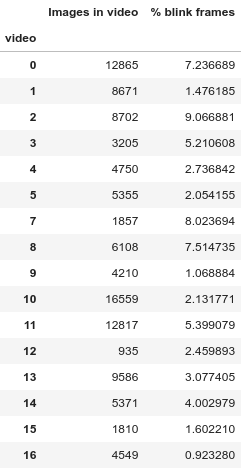
\includegraphics[width=0.3\textwidth]{drtA5y}
        \caption{Tabla con imágenes por video y porcentaje de parpadeos por video}
    \end{wrapfigure}

    Se parte el dataset en tres particiones.
    Una partición de entrenamiento, otra de validación y otra de test.\\
    Primero se parte el dataset en dos partes, entrenamiento y test, dejando el 20\% del dataset para test.
    Un valor de 20\% es relativamente generoso para el problema donde normalmente se considera un valor entre 10\% y
    20\%.

    Por ejemplo una competición como Imagenet tienen un 15\% del dataset como test\cite{imageNet}.
    La partición se hace mediante selección aleatoria ya que se considera que la selección estratificada no es
    necesaria ya que el dataset tiene una distribución de clases en cada video relativamente similar.
    Esto deja alrededor de 20.000 imágenes para test.\\
    En la partición de entrenamiento
    
    \subsection*{Generación de modelos}
    Para la resolución del problema se necesita un modelo que contenga dos entradas, una por cada ojo, y una salida,
    parpadeo o no. La aproximación obvia es tratar de utilizar un modelo preentrenado ya que permitiría ahorrar tiempo
    de entrenamiento comparado a un modelo inicializado sin preentrenamiento. Se procede a utilizar el zoo de Keras\cite[Insertar?cita?keras]
    ya que contiene una variedad interesante de modelos preentrenados en grandes datasets como Imagenet.
    El problema del zoo de Keras es que no tiene ningún modelo que use dos entradas. Se podría entrenar un modelo desde
    una inicialización random pero es sabido que el preentrenamiento suele llegar a una solución válida antes.
    
    Para utilizar el modelo preentrenado se crea un modelo con dos entradas donde cada entrada es seguida de un
    extractor de características seleccionado del zoo de modelos. Después la salida de los dos modelos es concatenada
    para ser conectada a una serie de capas totalmente conectadas.
    
    Esta arquitectura permite utilizar dos entradas pero también un modelo preentrenado así podemos converger a una
    solución más rápidamente.
    
    En la primera versión se usa un modelo VGG16 preentrenado en imagenet en cada rama para después añadir 2 capas
    totalmente conectadas: la primera con 128 nodos y la segunda con 1 ya que es la salida. El modelo en total contiene 
    29.560.705 parámetros.
    
    La segunda versión utiliza DenseNet121 también preentrenado en imagenet. La arquitectura es similar a la anterior c


    \section{Resultados}


    \section{Conclusiones}

    \newpage
    \bibliographystyle{plain}
    \bibliography{refs}
\end{document}
